\chapter{Il linguaggio}

Il linguaggio che stiamo proponendo è strutturato in 2 parti, e quindi due tipi di
file, che corrispondono al concetto di modello e layout; non a caso l'estensione
del primo è u2sm e il secondo è u2sl.

Il file modello sarà il contenitore delle definizione delle classi mentre nel
file layout il programmatore indicherà l'aspetto grafico del diagramma che si va
a generare.


\section{Model}

Il modello (estensione .u2sm) conterrà quindi tutte le informazioni riguardo il
contenuto/i dati
degli elementi che sarà possibile inserire in un diagramma in un secondo
momento. 

In un linguaggio ad oggetti uno degli strumenti fondamentali è la suddivisione 
delle classi sotto forma di package. Nella nostra proposta un file di modello
può contenere o una lista di classi (non associate ad un package) oppure una
lista di package.

La definizione del package (come un po' tutto il nostro linguaggio) è 
ispirata alla sintassi dei linguaggi java like.

\begin{lstlisting}[caption={Dichiarazione di package}, style={model}]
package nome.pkg{
	...  	
}
\end{lstlisting}

Nella definizione della classe è invece dichiarato in modo esplicito la
suddivisione tra i componenti base di una classe; sono quindi esplicitati quali
sono gli attributi, i metodi e le relazioni. L'aggiunta delle relazioni rispetto
ad una classica definizione di classe è necessaria per poter rappresentare nel
diagramma le frecce di collegamento.


\begin{lstlisting}[caption={Dichiarazione di classe}, style={model}]
class NomeClasse{
	relations{
		...
	}
	attributes{
		...
	}
	methods{
		...
	}
}
\end{lstlisting}

E' anche possibile dichiarare delle Interfacce utilizzando la parola chiave
interface al posto di class. 

\begin{figure}[htp]
\begin{center}
  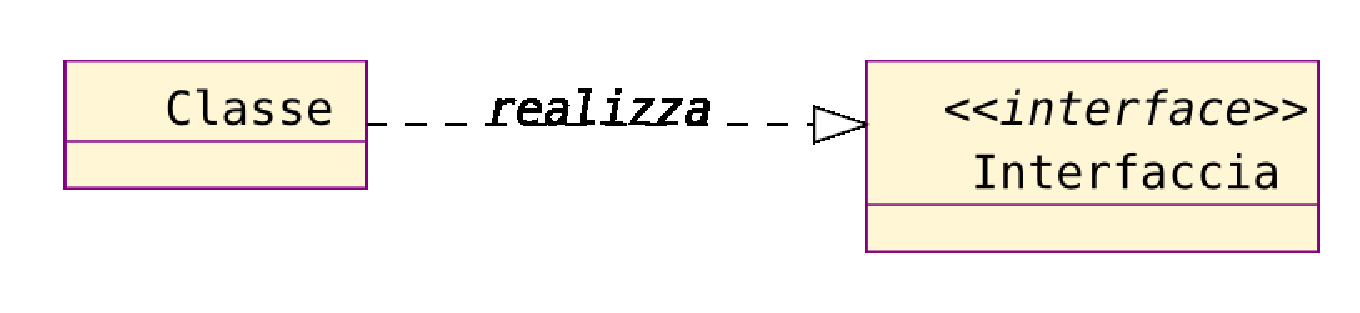
\includegraphics[width=0.8\textwidth]{img/class_interface}
  \caption[labelInTOC]{La visualizzazione di una classe vuota e di
  un'interfaccia vuota}
\end{center}
\end{figure}


Analizziamo ora il contenuto delle varie sezioni.

\subsection{Relazioni}

Nella sezione delle relazioni
viene appunto dichiarata una lista di definizione che contiene il tipo della 
relazione, una lista di classi (complete di package) 
con cui creare una relazione del tipo scelto
per ogni classe 3 parametri opzionali (che possono anche essere vuoti) in cui
il primo parametro e l'ultimo possono essere utilizzati per la definizione delle
cardinalità, mentre il parametro opzionale può essere utilizzato per definire
una descrizione della relazione; queste stringhe andranno a posizionarsi sul 
disegno delle frecce.

\begin{lstlisting}[caption={Dichiarazione di relazione}, style={model}]
relations{
	extend nome.pkg.NomeClasse ("(1,*)" , 
				"descrizione relazione", "(1,1)" );
	use nome.pkg.NomeClasse1, nome.pkg.NomeClasse2;
}
\end{lstlisting}

La lista dei possibili tipi di relzione sono:
\begin{itemize}
  \item{use (uso);}
  \item{extend (ereditarietà);}
  \item{associate (associazione);}
  \item{include (inclusione);}
  \item{realize (realizzazione);}
  \item{depend (dipendenza);}
  \item{composed (composizione);}
\end{itemize}

Di seguito un digramma creato per visualizzare tutti i tipi di relazione.

\begin{figure}[htp]
\begin{center}
  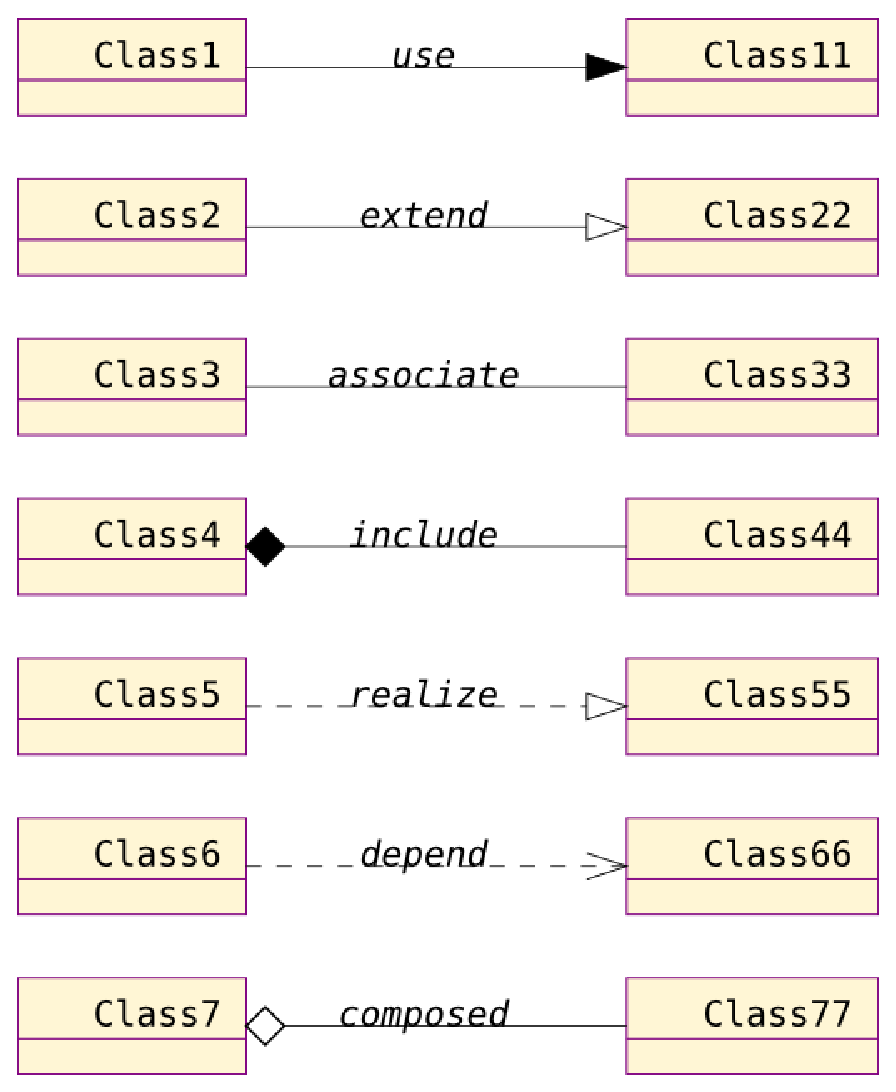
\includegraphics[width=0.5\textwidth]{img/relation_arrow}
  \caption[labelInTOC]{I vari tipi di relazione}
\end{center}
\end{figure}


\subsection{Attributi}

Gli attributi vengono dichiarati come visibilità:
\begin{itemize}
  \item public
  \item private
  \item protected
\end{itemize}

tipo (opzionale), nome attributo e valore di default (opzionale); la sintassi è
quella indicata nell'esempio sottostante.

\begin{lstlisting}[caption={Dichiarazione di attributi}, style={model}]
attributes{
	public int attr1=5;
	public "ArrayList<Integer>" attr2;
	private attr3;
}
\end{lstlisting}

Un ulteriore osservazione che si può fare è che i tipi (anche per i metodi e gli 
argomenti dei metodi) possono essere indicati come stringhe in modo da poter 
rappresentare situazioni con tipi contenenti caratteri speciali, come per esempio
un tipo ``generico''.

\subsection{Metodi}

Anche in questo caso la definizione dei metodi è del tutto simile alla
definizione della segnatura di un metodo in java.

\begin{lstlisting}[caption={Dichiarazione di metodi}, style={model}]
methods{
	public nomeMetodo1(int arg1=10, String arg2,arg3);
	private nomeMetodo2(arg1);
	nomeMetodo3();
}
\end{lstlisting}

Nell'esempio di definizione sopra riportato si possono contraddistinguere varie 
caratteristiche aggiuntive del nostro linguaggio; un metodo è caratterizzato
oltre che dal suo nome anche dal tipo di visibilità.

Gli attributi possono essere definiti sia con l'assegnazione di un tipo che con
la definizione del solo nome, c'è anche la possibilità di assegnare un valore di
default al parametro del metodo (caratteristica disponibile in alcuni linguaggi
tipo il PHP).
Possiamo notare il fatto che è possibile omettere gran parte degli attributi
perché l'idea è che deve essere obbligatorio definire solo gli elementi minimi
per poi poter indicare, opzionalmente, solo ciò che si vuole rappresentare nel
diagramma. 


\section{Layout}


Una volta specificato il modello si procede con il disegnare il diagramma
attraverso la definizione di un file di layout (estensione .u2sl).

Come prima cose bisogna associare al layout i modelli da utilizzare questa
operazione si effettua con il comando import; si possono importare più file
modello, ma devono essere importati come prime righe,altrimenti il compilatore
non sa cosa disegnare. E' possibile che ci sia il caso in cui la stessa classe è
contenuta in più file modello, la regola è che il primo dichiarato rimane; verrà
comunque segnalato un errore. Il percorso del file è un percorso relativo
rispetto al path in cui è salvato il file layout.

\begin{lstlisting}[caption={Import dei modelli necessari}, style={layout}] 
import test.u2sm;
\end{lstlisting}

La logica di definizione del modello si basa sul concetto delle scatole cinesi (o
dei gruppi); un gruppo viene definito attraverso l'uso delle parentesi quadre,
un gruppo può contenere altri gruppi o una definizione di classe.

Il codice sottostante definisce 2 gruppi; il primo contenente 2 sottogruppi e
 con una dichiarazione di classe per ogni gruppo di livello più basso.

\begin{lstlisting}[caption={Un semplice diagramma}, style={layout}] 
[
	[
		(class nome.pkg.NomeClasse1)
	]
	[
		(class nome.pkg.NomeClasse2)
	]
]
[
	(class nome.pkg.NomeClasse3)
]
\end{lstlisting}

In questo modo è molto semplice definire dei gruppi di oggetti da legare tra di
loro. Per ogni gruppo è possibile specificare delle proprietà subito dopo
l'apertura della parentesi che modificano l'aspetto del gruppo o delle classi in
esso contenute; le proprietà disponibili sono:

\begin{itemize}
  \item @layout i cui calori possono essere:
  \begin{itemize}
  	\item Nx* dove N è il numero di righe su cui disporre le classi;
  	\item *xN dove N è il numero di colonne su cui disporre le classi;
  	\item *x* per disporre le classi in un quadrato di lato uguale alla radice
  	quadrata del numero di elementi del gruppo;
  \end{itemize}
  
  \item @margin con quattro numeri che indicano il margine superiore (top),
  destro (right), inferiore (bottom), sinistro (left);
  \item @collapse che prende come parametri all, methods, attributes; per far in
  modo di non visualizzare i metodi o gli attributi o tutti e due;
  \item @hide-args che permette di nascondere gli argomenti dei metodi.
\end{itemize}

\begin{lstlisting}[caption={Diagramma decorato di attributi}, style={layout}] 
[
	[	
		@margin 15 10 5 0
		@collapse all
		(class nome.pkg.NomeClasse1)
	]
	[
		@collapse methods
		@hide-args
		(class nome.pkg.NomeClasse2)
	]
]
[
	@layout *x1
	@collapse attributes
	(class nome.pkg.NomeClasse3)
	(class nome.pkg.NomeClasse4)
]
\end{lstlisting}


Come è possibile notare dagli esempi di codice superiori l'introduzione di una
classe nel diagramma è dettata dal nome della classe circondato da parentesi
tonde all'interno di un gruppo.

Il nome della classe può essere indicato per esplicito inserendo il nome della
classe comprensivo di package oppure si possono inserire tutte le classi di un
package semplicemente indicando il package e facendolo seguire da un ``.*''.

Un semplice esempio esplicativo:

\begin{lstlisting}[caption={Diagramma decorato di attributi}, style={layout}] 
import test.u2sm;
[
	[	
		(class nome.pkg.NomeClasse1)
	]
]
[
	@layout *x*
	(class nome.pkg.*)
]
\end{lstlisting}

\section{Commenti}

I commenti possono essere inseriti in 3 modi:
\begin{itemize}
  \item /* \ldots */: dalla sintassi Java commento multilinea;
  \item // \ldots: sempre dalla sinstassi Java commento singola linea;
  \item \# \ldots: ulteriore commento singola linea.
\end{itemize}


I commenti vengono accettati in quasi tutti i punti del codice\footnote{Un
eccezione per esempio è la direttiva ``import''; in quel caso i commenti possono essere
inseriti solo dopo il ``;'', altrimenti vengono interpretati come appartenente
al percorso del path da importare.}.
